%%%%%%%%%%%%%%%%%%%%%%%%%%%%%%%%%%%%%%%%%%%%%%%%%%%%%%%%%%%%%%%%%%%
%                                                                 %
%                            CHAPTER THREE                        %
%                                                                 %
%%%%%%%%%%%%%%%%%%%%%%%%%%%%%%%%%%%%%%%%%%%%%%%%%%%%%%%%%%%%%%%%%%%

\chapter{CONCEPTUAL MODEL}\label{ch:model}

The goal of dataset versioning is to expose the relationships between versions of a dataset.
To do this, the concept model relates three kinds of objects, versions, attributes, and changes, using three different orientations.
The model obviously includes versions because they are the objects being compared.
However, identifying one object as a version of another does not give much insight into the nature of their relationship.
In order to characterize the change between two versions, the model relates their attributes.
The model uses the Dublin Core Term hasPart to facilitate the link from a version to its attribute.
The changes used then defines the difference between these attributes in each version.
The modeling process can be viewed as creating a mapping between an original set and a new dataset.
As mentioned previously, the operations conducted by data versioning systems boil down to primarily three operations: addition, invalidation, and modification.
Since these activities are so prevalent, we use these three procedures to characterize the relationships between versions.
A modification is straight forward to model because it maps together an attribute which exists in both versions, but addition and invalidation are a little different.
Because the attribute doesn't exist in one version or in the other for addition and invalidation, it forms a '0 to 1' relationship between the attributes.
This causes a problem conceptually because without a concept on one end, a mapping cannot be formed.
The chosen solution was to use the version concept as the anchor in place of the non-existant attribute.
This observation leads to the structure of the conceptual model used in this dissertation.
The nature of change can be determined by observing the construction used to model a relationship and counting the number of attributes on each side.
As a note, the figures in this chapter only depict the attribute relationships as 0 to 1, 1 to 0, and 1 to 1.
That is, the cardinality of links entering a change concept from an attribute to the number of links exiting to an attribute.
It is more valid to consider the relationships as 0 to X, X to 0, and X to Y in cardinality because it may take more than one attribute to identify an observation in a version.
For example, a cell in tabular data would need a row and a column to identify it, or a modification may change a single location attribute into two separate latitude and longitude entries.

An obvious concern about using these requirements to determine the mapping is that it does not guarantee meaningful versioning is being performed.
In order to ensure that the relationships being exposed by the mapping is valid, we must go back to the definition of versions.
Having common provenance establishes that performing a comparison between these two objects results in a relation pertaining to the same application.
In addition, if the objects also can share the same workflow step it establishes that they have relatable content.
This also addresses the possibility that we are comparing objects that have different purposes at separate points in a workflow, but share provenance as a result.
Therefore, before applying the methods in this model, it must be first established that the two objects satisfy the requirements to be versions of each other.

\section{MODIFICATION}

The simplest operation to model is Modification because it has no missing parts.
It maps a change from one attribute of version one to its corresponding attribute in version two.
In Figure \ref{ModificationFig}, a versioning comparison is being performed between two objects, Version 1 and Version 2.
Each version has an attribute, Attribute 1 and Attribute 2, respectively.
Finally, a change object connects the two attributes, denoting that the values described by the attribute are different.

Notice that the model captures neither the change's magnitude, nor the values of the attributes involved in the change.
These are not included because too much domain knowledge will be required to interpret the significance of the value.
In addition, the model would essentially begin storing a copy of the dataset, leading to space and redundancy concerns.
If an application needs to include this information, they can be added as a property of the attributes involved, but this is outside the scope of this thesis.
Simply knowing that the attribute has changed provides valuable information to identify the relationship between the two attributes from a versioning standpoint.
Sometimes it may be necessary to distinguish between modification changes.
For this reason, the change concept in this relationship may be sub-classed to differentiate between different kinds of change that map one attribute to another.
For example, in order to distinguish a modification in which the units of a measurement changes, a unit change concept, which sub-classes the modify change concept, can be used to connect the attributes from two different version.

The modification relationship is simple enough to understand, and a couple of well developed alternatives exist.
Schema.org supplies a subclass of the UpdateAction labeled ReplaceAction.
This concept has two properties, replacee and replacer which indicates that a new object replaces an old one.
This provides a structure very similar to the one found in Figure \ref{ModificationFig} with the only difference being the relationship between Attribute 1 and Change M reversed.
While this difference is subtle, it demonstrates a disagreement in view as to how change works in a system.
Schema.org's perspective looks at a single replacement action in isolation and models that quite well.
However, this versioning model views change as a quantity that flows through attributes from one version to another.
Unlike ReplaceAction, ModifyChange does not attribute changes to an actor, but rather it acts as a medium to convey change between objects.
PROV also has a property called isDerivedFrom to convey, "a transformation of an entity into another, an update of an entity resulting in a new one, or the construction of a new entity based on a pre-existing entity," \cite{Lebo2013}.
Changing this property into a qualified property then results in a form very similar to the construction in this model.
This should not be very surprising since the inspiration for the current form comes from the way PROV uses qualified properties.
It gains the advantage of turning the property into a concept that can be instanced and described easily using other ontologies.
The primary discrepancy between this versioning ontology and PROV-O is that Version 2 no longer needs to depend on a previous entity.
PROV assumes derivations to be part of a sequence, but situations exist, as seen in a later chapter, where research can create multiple simultaneous versions where an ordering does not matter.

\begin{figure}
	\centering
	\vspace{0.0in} % normally the command here would be \includegraphics
	%	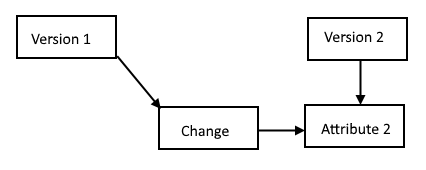
\includegraphics{figures/Addition.png}
	\begin{tikzpicture}[every node/.style={draw, rectangle}]
	\begin{scope}[node distance=20mm and 20mm]
	\node (c) [scale=1.25] at (1,0) {Change M};
	\node (1) [above left=of c, scale=1.25] {Version 1};
	\node (2) [above right=of c, scale=1.25] {Version 2};
	\node (a1) [below =of 1, scale=1.25] {Attribute 1};
	\node (a2) [below =of 2, scale=1.25] {Attribute 2};
	
	\draw [line width=2pt,->] (a1) -- (c);
	\draw [line width=2pt,->] (c) -- (a2);
	\draw [line width=2pt, ->] (1) -- (a1);
	\draw [line width=2pt, ->] (2) -- (a2);
	\end{scope}
	\end{tikzpicture}
	\caption{Model of the relationships between Versions 1 and 2 when modifying Attribute 1 from Version 1 as a result of Change M, resulting in Attribute 2 from Version 2}
	\label{ModificationFig}  % the \label command comes AFTER the caption
\end{figure}

\section{ADDITION}

In Figure \ref{AdditionFig}, the Addition model differs from the Modification construction by the absence of Attribute 1.
This should mean that there does not exist a relationship between Version 1 and the concept Change A as the inclusion of Attribute 2 into Version 2 does not in general use content from the previous object.
However, Change A in this model is not an activity, but a comparison relationship between Version 1 and 2.
Therefore, a path must exist from Version 1 to Attribute 2.
This formulation has the added benefit of conveying the idea of change as a quantity of flow, coming out of Version 1 and moving through the graph.
In this context, the structure establishes the left-hand version object as a source of flow when attributes become added to the following object.
This construction also forms a symmetric orientation with Invalidation.

In comparison, the AddAction from Schema.org considers addition as an activity performed by an agent.
This view of addition does not take into account the prior state of the collection being manipulated.
As a result, the proposed model for Addition should provide a better context for the relationships between objects when an attribute is added.
The corresponding concept in PROV-O is a Generation.
However, it relates together activities with entities, meaning that it could not relate together two versions or a version and an attribute.
This property also does not make sense because, once again, no activity is producing the versioning relationship.
Although, if we attribute new additions to the activity which generates Version 2, a relationship using Generation can be formed.
This formation, however, would also apply to other attributes added to Version 2, and convolute the role the activity took in an attributes generation.
In the versioning model used here, each added attribute connects to a particular change instance so that they can be individually described.

\begin{figure}
	\centering
	\vspace{0.0in} % normally the command here would be \includegraphics
%	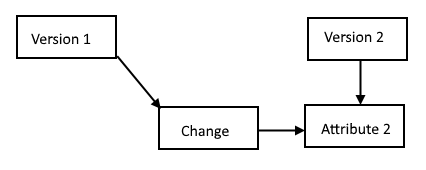
\includegraphics{figures/Addition.png}
	\begin{tikzpicture}[every node/.style={draw, rectangle}]
		\begin{scope}[node distance=20mm and 20mm]
			\node (c) [scale=1.25] at (1,0) {Change A};
			\node (1) [above left=of c, scale=1.25] {Version 1};
			\node (2) [above right=of c, scale=1.25] {Version 2};
			\node (a) [below =of 2, scale=1.25] {Attribute 2};
			
			\draw [line width=2pt,->] (1) -- (c);
			\draw [line width=2pt,->] (c) -- (a);
			\draw [line width=2pt, ->] (2) -- (a);
		\end{scope}
	\end{tikzpicture}
	\caption{Model of the relationships between Versions 1 and 2 when adding an Attribute 2 to Version 2 as a result of Change A}
	\label{AdditionFig}  % the \label command comes AFTER the caption
\end{figure}


\section{INVALIDATION}

The invalidation relationship has a missing attribute object on the other side of the relation, contrary to the addition construction.
As a result of the invalidation, an attribute no longer exists in the following version.
As seen in Figure \ref{InvalidationFig}, the invalidation change concept matches to the Version 2 object.
Just like in addition model, this construction maintains a link between the two version objects.
However, in this case, it makes more conceptual sense because Version 2 invalidates Attribute 1 by omitting it.

Related concepts include Schema.org's DeleteAction and PROV's Invalidation.
PROV defines the property as the "start of the destruction, cessation, or expiry of an existing entity by an activity," but since nothing actively creates versioning relationships, this property is inappropriate for this application \cite{Lebo2013}.
There is no activity to credit with removing the property in this comparison, and the absence results from a state-based property.
Schema.org defines the DeleteAction as, "The act of editing a recipient by removing one of its objects," \cite{SchemaRem}.
This definition assumes that an actor will perform an action upon an object or collection, removing one of its members, producing a new result.
This follows the provenance mentality, but when versioning, the resulting object has already been created.
Cases exist, as shown in Chapter 4, where an attribute is not included in a new version, thus indicating that it has been removed.
However, the most important point of contention in this definition is the idea of removal and deletion.
Although an object is no longer valid, it does not mean the data has been deleted.
Invalid data often gets removed, but this is not always the case.
As a result, naming the concept invalidation is more general and inclusive.

\begin{figure}
	\centering
	\vspace{0.0in} % normally the command here would be \includegraphics
	%	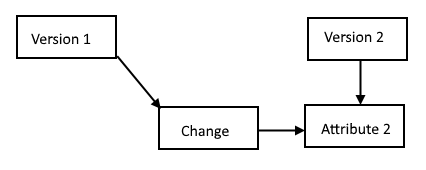
\includegraphics{figures/Addition.png}
	\begin{tikzpicture}[every node/.style={draw, rectangle}]
	\begin{scope}[node distance=15mm and 20mm]
	\node (c) [scale=1.25] at (1,0) {Change I};
	\node (1) [above left=of c, scale=1.25] {Version 1};
	\node (2) [above right=of c, scale=1.25] {Version 2};
	\node (a) [below =of 1, scale=1.25] {Attribute 1};
	
	\draw [line width=2pt,->] (a) -- (c);
	\draw [line width=2pt,->] (c) -- (2);
	\draw [line width=2pt, ->] (1) -- (a);
	\end{scope}
	\end{tikzpicture}
	\caption{Model of the relationships between Versions 1 and 2 when invalidating Attribute 1 from Version 1 as a result of Change I}
	\label{InvalidationFig}  % the \label command comes AFTER the caption
\end{figure}
